\chapter{Concept}\label{sec:concept}

    % \begin{blockquote}
    %     \paragraph{Intent:} General reminder and answer of RQ's 111111
        
    %     Structure:
    %     \begin{description}
    %         \item[1. Surrogates models combinations] Surrogate model is not universal. Domain-specific $\rightarrow$ Surrogate model portfolio 
    %             \begin{enumerate}
    %                 \item Surrogate model is not universal. Domain-specific $\rightarrow$ \textbf{Surrogate model portfolio}
    %                 \item Objectives have different complexity surface $\rightarrow$ Surrogate model is not universal $\rightarrow$ Describe objectives independently. \textbf{Heterogeneous/Composition surrogate model} 
    %             \end{enumerate}
                  
    %         \item[2. Dynamic sampling plan] Use sampling plan while surrogate is not valid
    %             \begin{enumerate}
    %                 \item Surrogate Validation. Stages and thresholds
    %                 \item Metrics
    %             \end{enumerate}

    %         \item[3. Scalability] Compositional surrogates in many-objective space
    %             \begin{enumerate}
    %                 \item Problem: Random solver on high dimensional space $\rightarrow$ Solution: Light surrogates 
    %                 \item Solving problem in subset of dimensions
    %                 \item Categorical parameters*
    %             \end{enumerate}

    %         \item[4. Discussion] General Conclusions. Infill criteria for Pareto-optimal solutions
    %     \end{description}
    % \end{blockquote}

    \epigraph{``All models are wrong but some are useful``}{\textit{– George Box}}

    This chapter introduces a general idea witch improve the limitations of model-based optimization.  

    As mentioned previously, fixed components can make the optimization process ineffective. That is why flexibility and variability must be introduced for each optimization step. Our concept focuses on the combination of surrogate models to effectively extrapolation required problems.


    %? The main objective of this part is to provide a thorough treatment of multi-objective parameter tuning with evolutionary algorithm(s)


    % The solution techniques and parametric selections however are usually problem-specific. \cite{abs181207958}
    % --------------------------------------------------------------------------------------------
    % ------------------------------------------------     RG1: Models combinations     
    % --------------------------------------------------------------------------------------------

    \section{Combinations of surrogate models}

        Let us address the main issue we have observed in multi-objective optimization. It considers that the solution techniques and parametric selections, however, are ordinarily problem-specific. Unfortunately, most surrogate model implementations are static. We tackle it with an improvement of a model variability \emph{in} a surrogate model(Compositional surrogate) and the extensibility \emph{with} surrogate hypotheses (Surrogate portfolio).

        % ------------------------------------------------     Compositional model       
        \subsection{Compositional Surrogate Model [RQ1]}
            The concept of the compositional surrogate means a combination of the multiple simple models that approximate the several objectives independently at the same time. Composite and conventional surrogates have a unified interface and together can implement a \emph{composite design pattern}, that let us operate with the individual and multi-objective surrogates uniformly. 

            Besides, a significant advantage of the compositional surrogate is a possibility to extend the single-objective parameter tuning to the multi-objective optimization. This provides the opportunity to reuse single-criteria models for multi-criteria optimization and dynamically reconstruct problem representation from mixed parts.
            Should consider that under \emph{compositional model} we mean a surrogate model that combines \emph{various} sub surrogates models for each optimization objective. The \emph{surrogate hypothesis} refinement is also used to emphasize on the fact that the surrogate model can completely describe all criteria from the objective space.

            % Nonetheless, the surrogate model is not universal to describe objectives independently. 

            The compositional surrogate has multiple opportunities for variability that outperform static models in adaptation to a real black-box problem. For example, choosing a specific set of models is a representation of knowledge about the subject area. If expectations during optimization are not met, the compositional model can be partially updated with saving time and effort while the static model needs to be completely replaced. The reasons for such changes might be the newly obtained results or might be the increased dimensionality of optimization space.

            % ------------------------------------------------     Scalability     
            \subsubsection{Scalability}
            The ability to scale the optimization solution could be considered as an adaptation to an unknown problem. Scalability, in this case, means perform the problem with high dimensions in parameters and objectives spaces.

            Practically showed that scalability is a problem for surrogate models and optimization algorithms also. As an illustration, popular surrogate models such as Gaussian process regression (Kriging) \cite{JonesSW98} struggle from high dimensional samples but provide excellent results in smaller dimensions. Also, the multi-objectives optimization algorithm has drawbacks in many-dimensional problems. Therefore, another advantage of the composite surrogate model is evident, which provide variability for extrapolation scalable search space.

            % % -------------------------     Categorical parameters      
            % \subsubsection{Categorical parameters} 
            %     Multi-objectivity and categorical parameters are essential for real parameter tuning. On the one hand, most related works used native models that support simulation with categorical features because it is interpretative and intuitive \cite{HutterHL11, nardi2019practical}. On the other hand, the feature-encoding methods are used to turn the categorical parameter into numbers for the generic model class. Coding features for a surrogate model can transform those in a meaningful form, that a model can use to perform calculations. Based on this samples interpretation, the model might extrapolate all points in the parameter space. Several types of encoders can be used to transform any mixed parameter types into a digital representative form.
            
        
        % ------------------------------------------------     Portfolio      
        \subsection{Surrogate model portfolio [RQ2]}
            In addition to the dynamic variability in the compositional surrogate, we combine several surrogate hypotheses in a surrogate portfolio to dynamically choose the one that is best suited to the specific problem. The unified interface and the ability to integrate models into a composite architecture make it possible to uniquely select and combine composite models side by side with static multi-objective models.

            Without problem's information, it is difficult to say which surrogate hypothesis would be better. Therefore, the model should be selected during optimization based on their usefulness (validity). The validation process involves checking the model for how well it assumes unknown data. For such validation evidence, a small portion of samples should be sacrificed. The test scores obtained from the separate test set are used to evaluate models accuracy and, accordingly, the quality of the possible corresponding solutions.
            The validation process allows us to evaluate surrogate models on information about how they summarize an unknown problem.
            
            For an optimization algorithm, a portfolio can be considered as a single model or as a collection of models. This allows determining the additional requirements of which optimization algorithms are applied to which surrogate models and how to combine such solutions. Such dynamic variability makes multicriteria optimization process also scalable and flexible.
            
            % With the flexibility that provides a compositional system to combine several models, that is valuable to produce several variants of compositions from available surrogates. There are created many hooks to combine and solve surrogates models. These placeholders give flexibility to the combination of hypotheses, testing, and solving/optimization. Bagging or ensemble technique can be applied to both steps: the surrogate models and the optimization algorithms. 
            % This functionality requires validation criteria to discard those that are not valid and comparison metrics to range and combine the best ones.

            Besides, the surrogate portfolio does not limit to use the latest state-of-the-art optimization algorithms and surrogate models together. 

    % --------------------------------------------------------------------------------------------
    % ------------------------------------------------     RG2: Sampling plan     
    \section{Sampling plan [RQ3]}
        After surveying the aforementioned related works, we obtain that most of the approaches use a static sampling plan, that determines an optimal number of initial samples by an outside oracle. 
        But in most cases, we cannot receive any guidance on an unknown problem. Thus, we need a dynamic sampling plan which adapts to a specific use-case.

        The general idea of solving this problem lays in binding the sampling design to a surrogate model validation process. An optimization process is guided by sampling design while neither among surrogate models are valid (Figure \ref{fig:concept_sampling}). Validity means that surrogate approximation could be useful for efficient global optimization.

        % ==== Sampling plan
        \begin{figure}[h!]
            \centering
            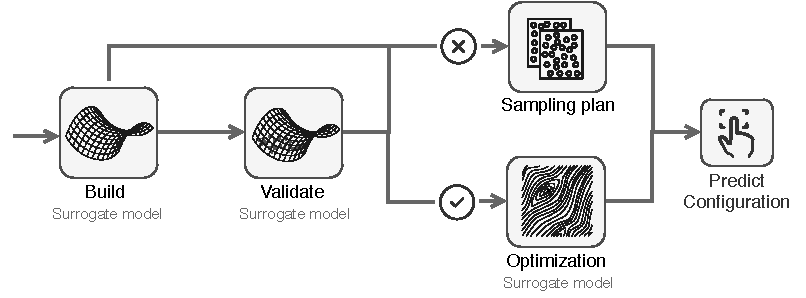
\includegraphics[width=\textwidth]{content/images/dinamic_sampling_plan}
            \caption[Non-dominated points]{Concept of a sampling plan dependency and model validation. A sampling plan is used if there is no valid model that can be useful for optimization purpose.} 
            \label{fig:concept_sampling} 
        \end{figure}      

        % -------------------------     Surrogate Validation      
        \subsection{Surrogate Validation}
        In the context of sequential model-based optimization, a common misconception lays in global model accuracy evaluation instead of the search space region of interest. That is why evaluation surrogate validity based only on the coefficient of determination(R2) is incorrect \cite{nardi2019practical}. Global accuracy metric can be used as a threshold value, exceeding which the model becomes not valid even with additional estimations.

        It is necessary to sacrifice a small portion of samples to check the surrogate model quality. Based on validation results, we can discard inadequate models and consider the solutions from valid models only. If neither model is valid, that the best decision now is a prediction from the sampling plan. This decision is repeated until a valid surrogate model is obtained.

        Validation should show how well the model extrapolates the available experiments (variance) and how well it can evaluate the data that is not seen (bias). The central concept for surrogate validation lays in the adaptation of best practices from machine-learning approaches for evaluation estimator's performance. 

        We are selecting surrogate models, based on accuracy shown on the test set, but selected models may not be correct if only one test set is taken into account for picking and models combination. Increasing surrogate complexity can mislead to represent wrong conclusions in a later stage of optimization (Figure \ref{fig:cv_overfitting}). This property cannot be neglected in evaluating a surrogate Validity. 


        % ==== train\valid\test
        \begin{figure}[h!]
            \centering
            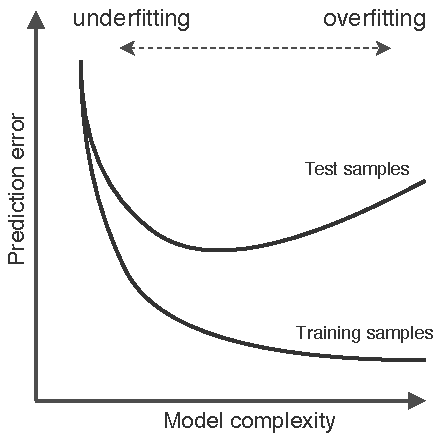
\includegraphics[width=5cm]{content/images/utility/cv_2x_test}
            \caption[surrogate validation: overfitting on the training set]{With rising model complexity overfitting on the training set becomes more likely \cite{HastieFT01, TobiasCV}.} 
            \label{fig:cv_overfitting}   
        \end{figure}

        
        It is necessary to manage the validation into phases with a separate test sats. This means that we need to select two separate test sets: the first one to select surrogate models; the second one to test those selected models.
        
            % if data split only to train/test set. There is a risk of over-fitting on the test data. It means that the test set 'leak' information to train set and final metrics does not report on the surrogate achievement. 
        
        However, partitioning the available samples into three sets, are drastically reduce the number of points which can be used for learning the model. Moreover, results can depend on a selective random decision for the samples splitting. The solution is might be cross-validation(CV, Figure \ref{fig:cv}). This is a procedure that avoids a separate validation set and divides test samples to \textit{k} equal folds. Set of folds are used to train model and in \textit{k} rounds, a new fold selected as a test set. The performance measured by cross-validation is the averaged over the values computed in the loop. This approach can be computationally expensive but requires fewer samples. 

        % ==== train\valid\test
        \begin{figure}
            \centering
            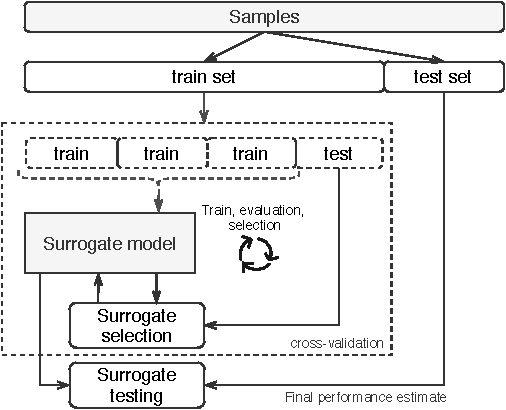
\includegraphics[width=10cm]{content/images/cv}
            \caption[Cross-validation: exploration vs exploitation]{Surrogates models validation. Cross-validation loop performs model selection based on global accuracy. Acceptable models are tested with focus on optimization region. } 
            \label{fig:cv}   
        \end{figure}
    

        To summarize it up, the model validation done in two stages:
        \begin{enumerate}
            \item \textbf{Cross-validation.} The overall accuracy of the surrogate model extrapolation is checked. Discard models that do not achieve the necessary precision threshold.
            \item \textbf{Surrogate testing.} The last check demonstrates the accuracy of the selected models and the corresponding assessment of possible solutions.
        \end{enumerate}
        
        The decision on which surrogate model is better done based on the information from all stages. If the model does not have a sufficient threshold, it is rejected as not valid. If there is no valid model, the assumption of the next configurations is accepted from the sapling plan. (Figure \ref{fig:concept_sampling}).

        % overfit - underfit
    
        % metrics comparison

    % --------------------------------------------------------------------------------------------
    % -----------------------------------------------------       Discussion      ----------------
    \section{Discussion}
        As answers for research questions, we propose the approach for dynamically combination surrogate models and dynamic sampling plan based on surrogate validation.
        \begin{itemize}
            \item \textbf{RG1:} For a dynamic combination of several surrogate models, it is necessary to implement a surrogate compositional model. This design allows for handling individual and compositional surrogate uniformly.
            \item \textbf{RQ:2} The combination of surrogate models in the portfolio is realized through the compositional model and stepwise validation.
            \item \textbf{RQ3:} The sampling plan is chosen to explore new random points when there is no valid model. This relation means that the sampling plan directly depends on whether we have a surrogate model that is capable of describing the optimization problem.
        \end{itemize}
         
        As a result, we extend the idea of classic \gls{smbo} with dynamic model selection and stepwise validation to obtain a multi-objective solution on various problem sceneries. 
        
        % To our knowledge, there exists no research that investigates how to make a composition of several different surrogate models and use it in a portfolio. We argue that the proposed concept from this thesis is the preferred choice for MBMO.























    % The usual optimization problem is a trade-off in producing the best possible multi-objective solution with less effort. Because we consider expensive function, an optimization effort, first of all, means evaluation budget. Each of these evaluations can require much time, energy, or other resources. That is why the main multi-objective comparison criteria are convergence to the Pareto frontier with a limited evaluation budget. 


    % It also takes into account the ratio of non-dominant solutions to the total number of measured configurations and their distribution on the Pareto frontier. In this thesis, under solving a multi-objective problem, we intend to find a set of none-dominated points that cover a wide range of objectives values and close as possible to the real Pareto front. 
    
    % If evaluations of the problem are expensive, the real count of experiments could be reduced throw applying a multi-objective algorithm on a surrogate model. This technique is the preferred choice for functional optimization when the evaluation cost is high.

    % While multiple algorithms could be applied, we selected \gls{moea} as default optimization techniques for the surrogate models. The advantage of \gls{ea} is that it could be easily modified and it could operate on a set of solutions candidates, that are well-fitted to approximate the Pareto-front. Finally, evolutionary algorithms can estimate highly complex problems in various use-cases.





        % -----------------------------------------------------      Infill criteria       
        % \paragraph{}{Infill criteria}
        % In the case of MOEA, solution of algorithm present as non-dominated final population. Based on unbiased, multi-objective criteria, they all uniformly could be presented as a prediction to the next evaluation. They represents current solution based on the surrogate model. Nevertheless, there is prior knowledge available in samples which can be taken into account. To reduce the number of candidates in the population, it is possible to deny those in which the distance to the nearest available sample is less than their average distance.
        % So there are two strategies for predicting from a population:
        % \begin{itemize}
        %     \item Prior and posterior knowledge. Based on changing metrics in available and proposed solutions
        %     \item Posterior knowledge. Proposed solutions are all equal
        % \end{itemize}


        
        % -----------------------------------------------------       Conclusions       
        % Also, to the best of our knowledge, has not been previously or stingy reported in the efficient multi-objective optimization.
        % Contribution:
        % \begin{itemize}
        %     \item Surrogate combination/composition with heterogeneous models
        %         \begin{itemize}
        %             \item Surrogate models portfolio
        %             \item Compositional surrogate model
        %             \item Combination of different(orthogonal) solvers
        %         \end{itemize}
        %     \item Surrogate portfolio. Search a better hypothesis  for a specific problem at a particular stage of parameter tuning
        %     \item Metric combination for evaluation Pareto optimal points
        %     \item Samples size depends on model(s) validity
        %     \item Concepts
        %         \begin{itemize}
        %             \item Combination of different(orthogonal) solvers
        %             \item Infill criteria for prediction selection
        %         \end{itemize}
        % \end{itemize}


        % structures include more than one possibility, as described above. Nevertheless, this level

        % Finally, another aspect worth mentioning is the fact that GSM appears in more than one cell. Indeed, hybrid methods


        % where the algorithms are allowed to query an oracle for additional data to infer better statistical models


        % They also reported that a speedup of a factor of 10 can nevertheless be obtained.



        % With multiple models, their flaws can combine, as well as the time required to build the models. In memetic algorithms, especially if the surrogate model is not very accurate, a local optimum can be found instead of the global optimum. But in terms of parameter tuning, this point should be better than a predefined sampling plan. Evaluation of this prediction improve surrogate model quality in the near-optimal area and improve prediction in the next round.
        % We could describe compositional-based surrogate optimization as compound grey-box system whit a lot of open research areas where surrogate should improve, managing portfolio, compare of predictions Pareto fronts. 
        % As a developer, you can be focused on a specific problem and don't know how to implement other components. This is one of the main advantages of the described approach.

        % less prone to overfitting
        % To our best knowledge, we are the first to make this simple observation, which can be applied to improve any Bayesian hyperparameter
        % optimization method.